\documentclass[conference]{IEEEtran}
\pdfsuppressptexinfo=-1
\pdfinfoomitdate=1
\pdftrailerid{}
\usepackage[utf8]{inputenc}
\usepackage[T1]{fontenc}
\usepackage{graphicx}
\usepackage{booktabs}
\usepackage{url}
\usepackage{cite}
\usepackage{amsmath}
\usepackage{xcolor}
\begin{document}

\title{Securing UAV Command and Control Against Quantum Adversaries: Hybrid, KEM Authenticated and Signature Based Post Quantum MAVLink Designs Compared on RISC-V Cores and ArduPilot}
\author{\IEEEauthorblockN{Anonymous author(s)}\IEEEauthorblockA{Affiliation withheld for review}}
\maketitle

\begin{abstract}
Drone flight controllers fielded today may still fly when an attacker can break classical public key cryptography. This measurement study compares six MAVLink command channel designs under one set of conditions: MAVLink 2 signing with a provisioned key, a classical session (X25519, Ed25519), a post quantum only session (ML-KEM-768, ML-DSA-44), a hybrid session of both, a session authenticated by pinned static ML-KEM-768 keys (design K), and an ML-DSA-44 signature on every command. In cycle accurate simulation of two open RISC-V cores, the hybrid session costs 1.75 to 1.89 times the vehicle side computation of the classical session and design K 1.03 to 1.13 times. Gateways that execute the cryptography in front of ArduPilot in software in the loop, over an emulated telemetry radio, show that a session keeps the per command cost of the shipped tag and misses almost no more commands than no authentication, while a signature per command misses the 0.5~s deadline for most commands (0.418 acknowledged in time; 0.851 within 1~s). A strict counter rule misses \mbox{+1.60} more commands per mission after outages, and still \mbox{+0.95} when it resynchronises inside the session; a replay cache misses none more than the published rule. In ProVerif, a replay cache gives injective agreement on commands only if each counter is checked and recorded in one step, and design K loses key secrecy once ML-KEM alone is broken. The code, data, logs and scripts are in a public repository whose link is withheld for review.
\end{abstract}

\section{Introduction}
A small multirotor runs its flight stack on a microcontroller and receives commands over a telemetry radio of tens of kilobits per second. MAVLink 2, the common protocol, offers a per message tag with a pre shared key \cite{mavsign}; without it, commands can be injected from the radio side \cite{kwon18,koubaa19}, and key establishment and endpoint authentication are left to the operator. A pre shared key is not broken by a quantum computer, but one stolen key exposes every past and future session that used it, and a fleet must provision and rotate such keys by hand; our model of a provisioned key with fresh nonces finds no forward secrecy for that reason. A session key exchange removes both problems, but its public key part is what a quantum computer threatens during the years a vehicle stays in service. The replacements are standardised: ML-KEM for key establishment \cite{fips203} and ML-DSA for signatures \cite{fips204}.

This is a measurement study, and its building blocks are known: design K follows KEMTLS with pre distributed keys and post quantum WireGuard \cite{kemtlspdk21,pqwg21}, the hybrid key derivation follows hybrid KEM combiners such as X-Wing \cite{xwing24}, and the replay cache is the sliding receive window of IPsec \cite{rfc4303}. Hyoung et al.\ argue from post quantum TLS handshakes over an emulated drone radio that, after the handshake, commands should carry only a symmetric tag, but derive rather than measure the per command cost \cite{hyoung26}. Missing is a comparison of complete designs on the same core, link and flight stack, including what the replay rule does to commands.

This paper contributes:
(1) executed baselines of six command channel designs on two open RISC-V core designs in cycle accurate register transfer level (RTL) simulation, with correctness checks, intervals over 15 runs, stack and code size, under one compiler and pinned libraries (Section~\ref{sec:rtl});
(2) a gateway emulation in front of ArduPilot software in the loop (SITL) that executes the handshakes, tags and replay rules on paired seeds (Section~\ref{sec:sitl});
(3) ProVerif models of the hybrid and the KEM authenticated sessions and of replay rules that accept out of order delivery, with the bounds of each model (Section~\ref{sec:formal}).
Every number in this paper is read by script from a committed result file.

\section{Related work}
\label{sec:rw}
Primitives are benchmarked on Cortex-M4 with pqm4 \cite{pqm4}, with stack optimised Dilithium \cite{greconici21} and with RISC-V extensions \cite{alkim20,fritzmann20}. Post quantum TLS has been measured on embedded clients \cite{burstinghaus20} and under packet loss \cite{paquin20,sikeridis20}; KEMTLS \cite{kemtls20,kemtlspdk21}, post quantum WireGuard and post quantum Noise \cite{pqwg21,pqnoise22} authenticate by encapsulation instead of signatures. For drones, MAVSec encrypts MAVLink \cite{mavsec19}, Ahmed et al.\ combine two ML-KEM-768 encapsulations with ML-DSA-65 certificates and compute radio times without a flight stack \cite{ahmed26}, and de Meneses et al.\ verify a post quantum EDHOC variant with estimated costs \cite{meneses26}; for vehicle to vehicle messages, frame loss can decide practicality \cite{twardokus24}. Table~\ref{tab:rw} compares methods, not figures, because platforms and links differ.

\begin{table*}[t]
\centering
\caption{Closest prior work and this paper (as recorded from each source)}
\label{tab:rw}
\setlength{\tabcolsep}{2pt}
\footnotesize
\begin{tabular}{llllll}
\toprule
Work & Platform & Link and stack & Per command cost & Availability & Formal check \\
\midrule
\cite{hyoung26} & x86 laptop & emulated UAV radio, TLS 1.3 & derived, not measured & not reported & none reported \\
\cite{burstinghaus20} & Cortex-A53, ESP32, others & Ethernet or Wi-Fi, network excluded & not reported & not reported & none reported \\
\cite{kemtls20,kemtlspdk21} & server or host & emulated network, TLS variants & not reported & not reported & proof on paper \\
\cite{pqwg21} & virtual machines & virtual network, WireGuard & not reported & not reported & Tamarin, with replay \\
\cite{ahmed26} & x86 laptop & none; SiK radio times computed & not reported & not reported & proof on paper \\
\cite{meneses26} & modelled Cortex-M4 & UAV, EDHOC variant, computed delays & not reported & not reported & Tamarin \\
\cite{twardokus24} & V2V chipset & DSRC, simulated and on road & measured & frame loss ratio & proof on paper \\
This paper & two RISC-V cores (RTL) & emulated SiK radio, ArduPilot SITL & executed (RTL) & measured per rule & ProVerif \\
\bottomrule
\end{tabular}
\end{table*}

\section{Threat model and designs}
\label{sec:design}
\emph{Threat model.} The attacker controls the radio: it reads, drops, delays, reorders and injects frames and replays old ones, and it may hold a quantum computer during the service life of the vehicle. Endpoints, their long term keys and the flight stack are trusted; side channels, jamming beyond the modelled loss and outages, and the confidentiality of commands are out of scope. So is resource exhaustion: an injected first flight makes the vehicle compute for 103~ms (design K) or 66~ms (hybrid) at the applied clock before anything is authenticated, so a deployment needs rate limiting. The goals are mutual authentication of the session endpoints, secrecy of the session key that keys the tags, and injective agreement on commands: every accepted command was sent by the ground station in that session and is accepted at most once. Per message protection stays the MAVLink 2 tag, SHA-256 over key, frame and counter truncated to 48 bits \cite{mavsign}, so a forged frame succeeds with probability $2^{-48}$, and every attempt must be sent over the radio.

\emph{Session designs.} All sessions end with the MAVLink 2 signing field of 13~B per message, keyed by the session key. \emph{Classical}: X25519 key exchange, Ed25519 signatures by both sides over the transcript and both identities, key confirmation tags. \emph{Post quantum only}: ML-KEM-768 and ML-DSA-44 in the same roles. \emph{Hybrid} (proposed): X25519 and ML-KEM-768 together, the session key derived from both secrets and a transcript hash, ML-DSA-44 signatures by both sides; a variant in which only the ground station signs leaves the vehicle unauthenticated in our model, so the vehicle signs too (mutual signing). \emph{KEM authenticated} (design K): each side holds the other's static ML-KEM-768 key; the ground station sends an X25519 share, an ephemeral ML-KEM-768 key and an encapsulation to the vehicle's static key, the vehicle answers with its share, a ciphertext to the ephemeral key, an encapsulation to the ground station's static key and a confirmation tag, and the ground station confirms; there are no signatures. Fig.~\ref{fig:flows} shows the flights of the hybrid session and of design K with their payload bytes; the classical and post quantum only sessions carry 224~B and 7,144~B in four flights, without MAVLink framing.

\begin{figure}[t]
\centering
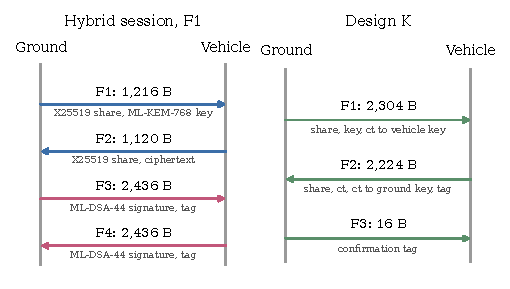
\includegraphics[width=\columnwidth]{fig_flows.pdf}
\caption{Handshake flights of the hybrid session with mutual signing (left) and of design K (right), with the bytes each flight carries as built by the executed protocols. Pink arrows carry ML-DSA-44 signatures; design K has none.}
\label{fig:flows}
\end{figure}

\emph{Baselines without a session.} \emph{Signing as shipped}: a provisioned key, no handshake. \emph{Signature per command}: an ML-DSA-44 signature on every command, verified by the vehicle; as in earlier per command designs it carries no counter, so it does not resist replay and is weaker than the sessions; a second variant adds a 6~B counter under the published rule, so it resists replay.

\emph{Replay rules.} MAVLink 2 signing carries a 48 bit timestamp per stream, and its \emph{published} rule accepts a frame whose timestamp exceeds the last one accepted on that stream \cite{mavsign}; our gateways put a per session counter into that field and apply the same rule, so gaps are allowed. The \emph{strict} rule accepts only the next counter; when the ground station's link layer gives up a frame, or when the vehicle sees a later counter and the next one does not arrive, the two sides resynchronise, either by a full new handshake or, in the second variant, by one authenticated message each way under the existing session key. The \emph{replay cache} accepts any counter not yet accepted within a window of 64 counters, the default receive window of IPsec \cite{rfc4303}.


\section{Method}
\label{sec:method}
\emph{RTL simulation.} Ibex in its small configuration \cite{ibex} and CV32E40P \cite{cv32e40p}, both RV32IMC without caches or wait states, are simulated cycle accurately with Verilator. One firmware image per design runs the vehicle and the ground side, each step timed with the cycle counter, 15 runs per session image with a fixed seed block (5 for the deterministic tag image); every run checks that both sides derive the same key, that all signatures and tags verify, and hash known answers; medians carry 95\% intervals over runs. Libraries are pinned and unmodified: mlkem-native \cite{mlkemnative}, mldsa-native \cite{mldsanative} and Monocypher \cite{monocypher}, all portable C, compiled with one compiler at \texttt{-O3}. Peak stack is measured by stack painting and includes the harness; code size is the text section of each image with unused sections removed, both sides and the harness included.

\emph{Gateway emulation with ArduPilot SITL.} ArduPilot Copter 4.7.2 \cite{ardupilot} flies a scripted mission of about 48~s (take off, two legs, land) with its built in vehicle model; the ground station sends one acknowledged COMMAND\_LONG message per second. A relay emulates a SiK class telemetry radio of 64~kbit/s with independent frame loss of 0.02, link layer retransmission that can deliver frames out of order, and one outage per mission starting 15--40~s after arming with an exponential duration of mean 5~s; an outage longer than 10~s tears the session down. A gateway pair between the ground station, the relay and the flight stack executes the handshake, the tags and the replay rule with the same algorithms (Python cryptography and host builds of the same libraries); the flight stack itself runs unmodified and never executes the cryptography. Vehicle side operations are released after a delay equal to their Ibex cycles at 168~MHz, the clock of a Cortex-M4 flight controller, fixed from the first runs before the flights (for design K, flown later, from the medians of all runs); ground side compute runs at host speed. The configurations fly 20 missions each on the same seeds, so they see the same outages; mission lengths differ slightly, so the number of commands per configuration ranges from 958 to 972. We therefore compare configurations by the commands missed per mission, paired by mission, with bootstrap intervals over missions. The host was slower than the applied delay for 3,979 of 254,813 vehicle side tags (at most 1,284 in one configuration); these are counted, not corrected.

\emph{Formal models.} ProVerif \cite{proverif} checks secrecy, agreement and reachability under a Dolev Yao attacker with perfect abstract primitives and unbounded sessions; binding properties of the KEMs are not analysed. Session models carry one command, a rekey and a further command per session; replay cache models carry three commands per key; the bounded window is modelled on the command layer for a window of two counters, not the 64 flown. Rekey grace periods, counter wrap and timestamps are not modelled. Breaking a component is modelled by giving its secrets to the attacker.

\emph{Discipline.} Of 12 technical predictions hashed before the runs and scored by script under the less favourable reading, 10 hit, 1 fell between and 1 missed; the thresholds were broad, and design K was added after registration.

\section{Executed baselines on core designs}
\label{sec:rtl}
Table~\ref{tab:rtl} gives the cost of one session start and of one command. On CV32E40P the hybrid session costs 1.75$\times$ [1.59, 1.77] the classical vehicle side, and on Ibex 1.89$\times$ [1.72, 1.91]; on the ground side, which signs first, the ratios are 1.92$\times$ and 2.09$\times$. Against the post quantum only session the hybrid costs 1.26$\times$ [1.05, 1.41] on the vehicle side and 1.55$\times$ on the ground side of CV32E40P. The two designs differ by two X25519 operations, a fixed 6.32~M cycles, yet their measured medians differ by only 4.48~M: ML-DSA-44 signing repeats with rejection and took 5.6 to 39.2~M cycles per signature, so the medians of the signing designs are noisy, and the sums of primitive medians drawn in Fig.~\ref{fig:rtl} exceed the measured session medians. With Monocypher, one X25519 multiplication (3.16~M cycles on CV32E40P) costs more than an ML-KEM-768 encapsulation (1.70~M), and an Ed25519 verification 4.53~M; this is a property of one portable C library designed for size, and a faster classical library would raise every ratio over the classical session.
\begin{table}[t]
\centering
\caption{Executed baselines: million cycles per unit (RTL simulated, medians of 15 runs, 5 for the tag row) and code size on CV32E40P (host measured)}
\label{tab:rtl}
\setlength{\tabcolsep}{2.5pt}
\begin{tabular}{lrrrrr}
\toprule
 & \multicolumn{2}{c}{Vehicle} & \multicolumn{2}{c}{Ground} & Code \\
Design & Ibex & CV32E40P & Ibex & CV32E40P & (kB) \\
\midrule
MAVLink 2 tag$^{a}$ & 0.015 & 0.013 & 0.014 & 0.013 & 21.7 \\
Classical session & 15.5 & 12.4 & 15.4 & 12.4 & 44.9 \\
PQ only session & 23.8 & 17.3 & 21.6 & 15.4 & 56.1 \\
Hybrid session & 29.2 & 21.8 & 32.3 & 23.9 & 66.5 \\
KEM auth.\ session (K) & 17.4 & 12.8 & 20.2 & 14.7 & 46.0 \\
ML-DSA-44 per command$^{b}$ & 5.4 & 3.9 & 10.0 & 7.4 & 37.8 \\
\bottomrule
\end{tabular}

\smallskip\footnotesize Session rows: one session start. $^{a}$ check (vehicle) and generation (ground) of one tag over a COMMAND\_LONG frame. $^{b}$ verification (vehicle) and signing (ground) of one command.
\end{table}

\begin{figure}[t]
\centering
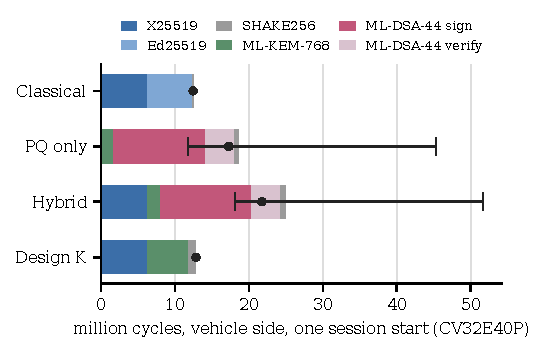
\includegraphics[width=\columnwidth]{fig_rtl.pdf}
\caption{Vehicle side cycles of one session start on CV32E40P by primitive (RTL simulated). Bars are sums of primitive medians, which exceed the measured medians of the signing designs; the whisker is the bar total if its one signature took the fastest or the slowest ML-DSA-44 signing observed; the dot is the measured session median.}
\label{fig:rtl}
\end{figure}
\begin{figure}[t]
\centering
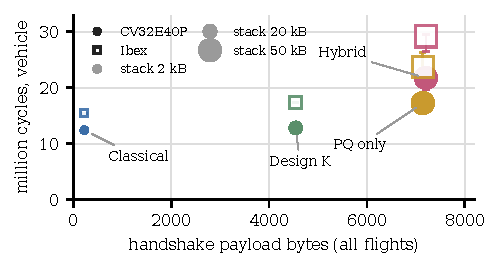
\includegraphics[width=\columnwidth]{fig_space.pdf}
\caption{Cost map of the session designs: vehicle side cycles of one session start (median with 95\% interval over runs, RTL simulated) against the payload bytes of all handshake flights. Filled markers CV32E40P, open markers Ibex; marker size grows with the peak stack (legend).}
\label{fig:space}
\end{figure}

Fig.~\ref{fig:space} places the four session designs by vehicle side cycles and handshake bytes. Design K avoids both ML-DSA-44 operations: on CV32E40P its vehicle side costs 1.03$\times$ the classical session and 0.59$\times$ [0.55, 0.65] the hybrid one, it needs 18.8~kB of stack against 50.5~kB for the hybrid (2.1~kB classical), and it carries 4,544~B in three flights against 7,208~B for the hybrid session, which carries 32$\times$ the bytes of the classical handshake. Code for both sides and the harness grows from 44.9~kB (classical) to 66.5~kB (hybrid) and 46.0~kB (design K). The 5 ArduPilot builds we measured leave 102 to 377~kB of flash and at least 111~kB of static RAM free (host measured from linker output), so the code fits, but a 50.5~kB stack would need a thread of its own or a stack optimised signer \cite{greconici21}; a vehicle only image was not measured. After the handshake a command costs a tag check of 13,314 cycles on a COMMAND\_LONG (the tag alone, without parsing); verifying an ML-DSA-44 signature on the same frame costs 292$\times$ as much on CV32E40P, and signing it on the ground side about twice that. Ibex needs 1.34$\times$ the cycles of CV32E40P for the same handshake, so cycle counts do not transfer between cores.

\section{Gateway emulation with ArduPilot SITL}
\label{sec:sitl}
\begin{table*}[t]
\centering
\caption{ArduPilot SITL behind the gateway emulation and an emulated SiK class radio, 20 paired missions per configuration}
\label{tab:sitl}
\setlength{\tabcolsep}{3pt}
\begin{tabular}{lrrrr}
\toprule
Configuration & Handshake (s) & Added round trip (ms) & Share acknowledged within 0.5~s [95\% CI] & Missed per mission \\
\midrule
No authentication & -- & ref. & 0.935 [0.902, 0.963] & 3.15 \\
MAVLink 2 signing as shipped$^{a}$ & -- & 4.0 & 0.932 [0.902, 0.962] & 3.30 \\
Classical session & 0.19 & 4.3 & 0.935 [0.904, 0.965] & 3.15 \\
Hybrid, published rule & 1.49 & 4.4 & 0.931 [0.896, 0.961] & 3.30 \\
Hybrid, strict rule, new handshake & 1.50 & 4.3 & 0.898 [0.858, 0.936] & 4.90 \\
Hybrid, strict rule, in session & 1.49 & 4.8 & 0.912 [0.872, 0.947] & 4.25 \\
Hybrid, replay cache & 1.44 & 4.2 & 0.932 [0.899, 0.964] & 3.30 \\
Design K, published rule & 0.92 & 4.7 & 0.934 [0.903, 0.964] & 3.15 \\
ML-DSA-44 per command & -- & 496.1 & 0.418 [0.374, 0.459] & 28.25 \\
ML-DSA-44 per command, counter & -- & 493.8 & 0.439 [0.403, 0.477] & 27.25 \\
\bottomrule
\end{tabular}

\smallskip\footnotesize Handshake: median from F1 until both sides hold the key (vehicle accepting F3 for design K, ground accepting F4 otherwise), emulated link and executed cryptography with RTL derived vehicle delays. Added round trip: median round trip to the flight stack's acknowledgement against no authentication (SITL measured). Acknowledged share and missed commands (not acknowledged within 0.5~s) include one outage per mission. $^{a}$ signing inside ArduPilot and the ground station at host speed, without RTL derived delays.
\end{table*}
\begin{figure}[t]
\centering
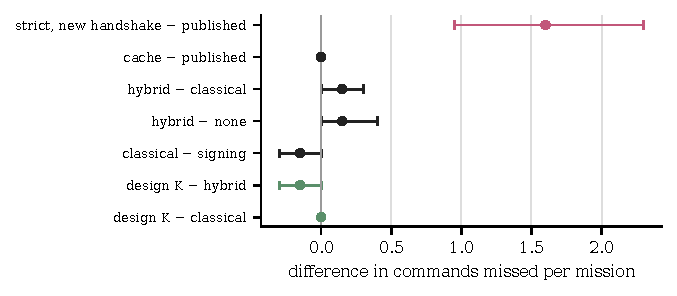
\includegraphics[width=\columnwidth]{fig_sitl.pdf}
\caption{Paired differences between configurations of the commands missed per mission (not acknowledged within 0.5~s, outages included), mean over missions with 95\% bootstrap interval (SITL measured). Negative values mean fewer missed commands than the reference.}
\label{fig:sitl}
\end{figure}
\begin{figure}[t]
\centering
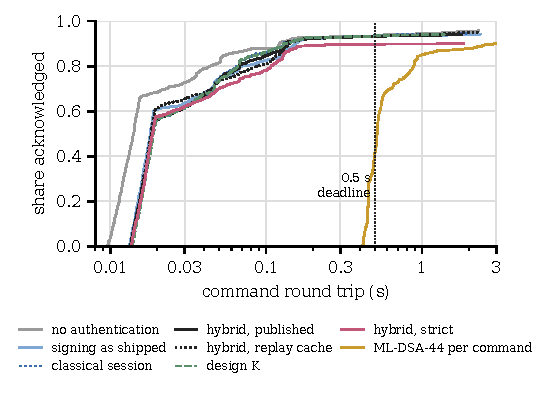
\includegraphics[width=\columnwidth]{fig_latency.pdf}
\caption{Distribution of the command round trip to the flight stack's acknowledgement over all missions (SITL measured); commands never acknowledged count as unbounded, so each curve ends below one. The dotted line is the 0.5~s deadline.}
\label{fig:latency}
\end{figure}
Table~\ref{tab:sitl} gives each configuration. Once a session exists, its per message cost is that of the shipped tag: the hybrid session adds 4.4~ms to the median command round trip, the classical session 4.3~ms and signing as shipped, which runs inside the flight stack without gateways, 4.0~ms. These milliseconds are mostly the airtime of the 13~B signing field: the median one way latency rises by 1.8~ms with signing as shipped, against 1.6~ms of airtime per direction at the radio rate, while the applied tag delays are 0.08 to 0.13~ms. The hybrid handshake takes 1.49~s over the emulated radio against 0.19~s for the classical session, a cost paid once per session, and design K completes in 0.92~s. Signing as shipped missed 17 commands that arrived after a newer frame and failed the shipped timestamp rule.

Fig.~\ref{fig:latency} shows the whole distribution of round trips. A signature on every command adds 496.1~ms to each round trip, mostly airtime of the 2.4~kB signature, since the applied verification delay is 32~ms; this puts the median round trip next to the deadline: 0.418 of its commands are acknowledged within 0.5~s, 0.636 within 0.55~s, 0.743 within 0.75~s and 0.851 within 1~s.

Fig.~\ref{fig:sitl} compares configurations by the commands missed per mission. Most session configurations differ in at most three of the 20 missions: the hybrid session misses \mbox{+0.15} commands per mission against no authentication (\mbox{+0.00} to \mbox{+0.40}, \mbox{2} missions differ) and \mbox{+0.15} against the classical session, a small cost from re-handshakes after long outages; design K and the classical session miss the same commands (\mbox{+0.00}). Link layer retransmission delivers some frames after newer ones (reordering depth up to 2), and the published rule rejected 11 of them as late; the replay cache accepted them, but they had already missed the deadline, so the cache misses exactly as many commands as the published rule (\mbox{+0.00}, \mbox{0} missions differ).

The strict rule is the one that costs commands. Resynchronising by a full new handshake, it misses \mbox{+1.60} commands per mission against the published rule (\mbox{+0.95} to \mbox{+2.25}; \mbox{0.033} of the acknowledged share), mainly through resynchronisation, not reordering: 58 commands were lost while no session existed during 12 resynchronisations, 10 of them triggered when the link layer gave up a frame during an outage, against 13 rejected as ahead of the expected counter; 12 of its missions restarted the session, against 1 under the published rule. Resynchronising inside the session removes the handshake but not the cost: across 22 resynchronisations it still misses \mbox{+0.95} commands per mission against the published rule (\mbox{+0.40} to \mbox{+1.55}), \mbox{-0.65} against the strict rule with a new handshake, because every command sent while the counter is out of step is rejected. Adding a counter to the signature per command does not change its availability (\mbox{-1.00} commands per mission, \mbox{-2.50} to \mbox{+0.30}).

\section{Formal results}
\label{sec:formal}
ProVerif checked 240 queries in 39 model files: 102 proved, 126 counterexamples, 3 that the tool could not prove and 9 that reached the time limit. Of the counterexamples, 71 are reachability checks that must fail: they show that a command or a session key can be accepted, so the agreement results are not vacuous. The others are found in designs before their fixes, in fallback and firmware update models not discussed here, in deliberate controls with a broken component or a missing check, and in the results below. With mutual signing the hybrid session keys stay secret and each side authenticates the other; the keys stay secret when either the classical or the KEM component is broken, and after a later theft of the long term keys. With ML-DSA-44 broken (both signing keys known to the attacker), authentication fails and an active attacker learns the key a side accepts; only a session that both sides accepted with the same key stays secret, which the X25519 and ML-KEM exchange still gives. The hybrid session's authentication therefore rests on ML-DSA-44 alone.

Design K keeps its keys secret when the classical component is broken and after a later theft of the static keys, and the vehicle authenticates the ground station. With ML-KEM broken, however, its keys are not secret: the attacker sends its own first flight with stolen static keys, and the X25519 share does not save the session against an active attacker, whereas the hybrid session still has its signatures; with its static keys known, design K fares like the hybrid session with ML-DSA-44 broken. Authentication of the vehicle by the ground station is proved only in a model in which static and ephemeral KEM keys have distinct types; the general model reached a time limit of 3~h without finding an attack or a proof.

For out of order delivery, a replay cache proves injective agreement on commands when the vehicle checks and records each pair of session and counter in one step and never forgets an entry, a condition stated in the model as a restriction, not derived. When concurrent branches read a table before either records, the model gives a counterexample, and a table read in sequence could not be proved; an implementation must therefore check and record atomically. A bounded window was proved only on the command layer for a window of two counters, and the published timestamp rule could not be proved.

\section{Discussion and limitations}
For streamed commands the results support a session: its post quantum cost is paid once, and the per command cost stays that of the shipped tag. Where both identities can be pinned, design K needs 0.59 of the vehicle side cycles and about a third of the stack of the hybrid session, at the price of resting secrecy and authentication on ML-KEM alone; the hybrid session keeps the classical component as a guard against a flaw in ML-KEM, while its authentication rests on ML-DSA-44. A signature per command, as measured here with ML-DSA-44, fits only commands that can wait about a second. The replay rule should be a replay cache that checks and records atomically: a strict rule costs commands after outages even when it resynchronises without a new handshake. A smaller signature such as Falcon-512 (666~B against 2,464~B per signed command here \cite{falcon}) would cut the airtime of a signature per command; it was not evaluated.

\emph{Threats to validity.} (i) Cycles come from two open core designs with single cycle memories, applied at a Cortex-M4 clock; Cortex-M flight controllers have flash wait states, caches and other multipliers, and an earlier run of portable C code on Ibex took 1.6 to 2.9 times the published portable C cycles on Cortex-M4 and 3.2 to 4.3 times its assembly for ML-KEM-768 and ML-DSA-44; stack optimised signing \cite{greconici21} or RISC-V extensions \cite{alkim20,fritzmann20} would change the figures. (ii) One classical library was measured, and it favours the post quantum designs. (iii) The cryptography runs in gateways, not in the flight stack, so the scheduling load of a handshake on the flight controller is not measured; vehicle compute is a delay applied per event without a busy processor, and the host was slower than that delay for a small share of tags. (iv) The radio is an emulation with independent frame loss and one scripted outage per mission, real loss is bursty, and the strict rule results rest on about a dozen outage triggered events. (v) Twenty missions per configuration, a bootstrap over missions that may under cover, and no correction for the several paired comparisons. (vi) The formal models use perfect primitives and small bounds (Section~\ref{sec:method}). Next, the baselines should be repeated on Cortex-M boards with the vehicle side inside the flight stack and a real radio.

\section{Conclusion}
Executed under one set of conditions, a hybrid post quantum session for drone commands costs 1.75 to 1.89 times the vehicle side computation of a classical session on these cores and many times its handshake bytes, yet keeps the per command cost of the shipped tag; a KEM authenticated session with pinned keys is the cheapest post quantum option but rests on ML-KEM alone, and a signature per command misses a 0.5~s deadline for most commands. The replay rule matters as much as the algorithms: a strict rule loses commands after outages, with or without a new handshake, while a replay cache loses none against the published rule and is safe only if it checks and records each counter in one step.

\bibliographystyle{IEEEtran}
\bibliography{references}
\end{document}
